%\documentclass[authoryear,5p]{elsarticle}
\documentclass[authoryear,preprint,11pt]{elsarticle}
\bibliographystyle{elsarticle-harv}
\usepackage{graphicx}
\usepackage{amsmath,amsfonts}
\usepackage{lineno}
\linenumbers
\usepackage{subfigure}
\usepackage[pdftex]{color}
\definecolor{darkblue}{rgb}{0,0,0.5}
\definecolor{darkgreen}{rgb}{0,0.5,0}
%\usepackage[pdftex, colorlinks, citecolor=darkblue,linkcolor=darkgreen]{hyperref}
\usepackage[pdftex, colorlinks]{hyperref}
\textwidth 6.75in
\oddsidemargin -0.15in
\evensidemargin -0.15in
\textheight 9in
\topmargin -0.5in
\newcommand{\ud}{\mathrm{d}}
\newcommand{\E}{\mathrm{E}}
\newcommand{\C}{\mathrm{Cov}}
\newcommand{\V}{\mathrm{Var}}

\newcommand{\cb}[1]{{\it \color{darkgreen} (#1)}}



\journal{\tiny Journal of the Royal Society Interface} 
\begin{document}
\begin{frontmatter}
  \title{Quantifying Limits to Detection of Early Warning for Critical Transitions}
  \author[cpb]{Carl Boettiger\corref{cor1}}
  \ead{cboettig@ucdavis.edu}
  \author[esp]{Alan Hastings}
  %\author[info]{}
  %\author[davis]{}
  \cortext[cor1]{Corresponding author.}
  \address[cpb]{Center for Population Biology, 1 Shields Avenue, University of California, Davis, CA, 95616 United States.}
  \address[esp]{Department of Environmental Science and Policy, University of California, Davis} 


  \begin{abstract}

Catastrophic regime shifts in complex natural systems may be averted through advanced detection. 
Recent work has provided a proof-of-principle that many systems approaching a catastrophic transition may be identified 
through the lens of early warning indicators such as rising variance or increased return times.  
Without the benefit of hindsight of a collapse, 
applications of these approaches must quantify how reliable different indicators are in avoiding false alarms, 
and how sensitive they are to missing subtle warning signs.  
We propose an approach which quantifies this trade-off between reliability and sensitivity, 
allows comparisons between different indicators, 
and estimates what data are necessary to achieve a desired error rate. 
We show these error rates can be quite severe for common indicators even under favorable assumptions, 
and illustrate how a likelihood-based indicator can improve this performance.  

  \end{abstract}

  \begin{keyword}
early warning signals \sep tipping point \sep alternative stable states \sep likelihood methods 
   \end{keyword}
 \end{frontmatter}

\section{Introduction}
There is an increasing recognition of the importance of regime shifts or critical transitions at a variety of scales in ecological systems~\citep{Holling1973, Wissel1984, Scheffer2001, Scheffer2009, Drake2010, Carpenter2011}⁠. 
Many important ecosystems may currently be threatened with collapse, including corals~\citep{Bellwood2004}, fisheries~\citep{Berkes2006}⁠, lakes~\citep{Carpenter2011}, and semi-arid ecosystems~\citep{Kefi2007}⁠. 
Given the potential impact of  these shifts on the sustainable delivery of ecosystem services
and the idea that management responses would be needed either to avoid an undesirable shift or else to adapt to novel conditions,
it is important to develop the ability to predict impending regime shifts based on early warning signs. 
With a good model of the system, detail-oriented approaches could be useful~\citep{Lenton2009},
but in cases where specific models are not available general approaches are needed~\citep{Scheffer2009}⁠.

\cb{Need more introduction defining critical transitions, early warning signals etc?}


\section{The summary statistics approach}
Foundational work on early warning signals has operated under the often-implicit assumption %often unstated?
that the system dynamics contain a saddle-node bifurcation and
looks for patterns that would be associated with approaching this bifurcation point.
The typical pattern has been a trend in a summary statistic such as
variance~\citep{Carpenter2006}, autocorrelation~\citep{Held2004, Dakos2008},
skew~\citep{Guttal2008}, spectral ratio~\citep{Biggs2009}.
% consider additional citations
While attractive for their simplicity, such approaches are subject to numerous challenges.
In this paper we argue for a model-based approach, 
and describe how this can be done in a way that best addresses these difficulties.

\subsubsection*{Arbitrary windows}
While superficially simple to use, the calculation of these statistics is subject to 
several arbitrary decisions and additional assumptions,
such as the choice of window size over which the statistic is computed,
the choice of detrending,
and whether and by how much the consecutive time-windows used in the calculation should overlap.  
\citet{Lenton2012} compare the performance of different approaches to these issues,
showing that choice of window and method used for detrending indeed influence the results,
and each approach considered has pros and cons.  
Without a consistent choice or a clear mechanism to determine one, % Should we say this part?
it is difficult to evaluate and compare between such methods.  
A model-based approach side-steps these issue entirely.  
\cb{
 Should we mention the ergodic problem here - that averaging over windows isn't averaging across time series, 
 and that it assumes stationarity, which is precisely the thing we're looking to change?  
 Similarly could mention that the detrending approaches can remove the signal?
 We could also mention that some popular approaches such as autocorrelation require evenly-spaced points,
 and interpolating is incorrect, introducing fictitious correlations?
}


\subsubsection*{No quantitative measures}
The warning signal, ``an increase in statistic $x$,'' is not quantitative,
making it difficult to compare between signals or to
attribute a statistical significance to the detection.
Some authors have suggested Kendall's correlation coefficient to quantify an increase~\citep{Dakos2008, Dakos20011} 
in autocorrelation or variance.  
Other measures of increase, such as Pearson's, have also been proposed~\citep{Drake2010}.  
Much of the literature using summary statistics simply forgoes quantifying
the increase or estimating significance.  
While this may be satisfactory in experimental systems with controls and replicates to compare to,~\citep[\emph{e.g.}][]{Drake2010, Carpenter2011}
any real-world application of early warning methods will not have the luxury of controls and replicates.
In such cases a quantitative definition of detection is essential.  
\cb{ We will see that correlation tests in summary statistics are an ineffective way to do this.  }


\subsubsection*{Problematic null models}
Specifying an appropriate null model is also difficult.  
Non-parametric null hypotheses seem to require the fewest assumptions but in fact can be the most problematic.  
For instance, the standard non-parametric hypothesis test with Kendall's tau rank correlation coefficient
assumes only that the two variables are independent, but this is
an assumption that is violated by the very experimental design:
since one variable is time and the other a moving time-averaged window.  
Under such a test any adequately large data set will find a significant result, regardless of whether a warning signal exists.
A similar problem arises when the points in the time series are reordered to create a null hypothesis -- 
this destroys the natural autocorrelation in the time series.  
\cb{I feel citing \citet{Dakos2011} and \citet{Dakos2008} for these two examples would be impolite\dots} 
Parametric null models have been more promising, and have brought us closer to a model-based approach where assumptions are explicit.  
For instance, autoregressive models~\citet{Dakos2008} have been proposed, which are first parameterized from the data.  
\cb{is this next line okay to leave in?}
Estimating the null models directly from the data using a maximum likelihood framework, will provide the most powerful basis for this test.  
\citet{Seekell2011} proposes a conditional heteroscedaticity as a summary statistic particularly because probability models for the null distribution are readily available.\cb{Though as a measure of changing variance, it suffers from the weaknesses mentioned above, but no need to mention that.} 


\cb{This is a particular concern given the tendency for warning signals to be found only in the largest data sets, 
which has been taken as evidence that large data sets are required for successful detection,
not that large data sets have higher false-positive rates under certain metrics.}
\cb{A similar problem exists with the proposal that large deviations from the running variance,
i.e. in excess of 2 standard deviations, be taken as evidence of an increase.
This likewise guarantees the false positive rate goes to unity as the number of observations increases.}



\subsubsection*{Hidden assumptions}
Assumes that the system sits effectively at equilibrium around a stable state  
and tests whether the system may be experiencing the slow change of a parameter that is weakening the stability of that state,
moving the system towards a saddle-node bifurcation.  
As such processes may be common in natural systems this is an important scenario to consider,
but without the clarity of assumptions made in a modeling approach there is a risk that
early warning signs will be used in situations where they do not apply.  


%Differing system dynamics
The underlying assumption that the system contains a saddle-node bifurcation
can be easily overlooked in summary-statistic based approach.  
For instance, variance may increase for reasons that 
do not signal an approaching transition~\citep{Schreiber2003, Schreiber2008}.
Alternatively, variance may not increase as a bifurcation is approached~\citep{Livina2012, Dakos2011a}.
Some classes of sudden transitions may exhibit no warning signals~\cite{Hastings2010}.   
While no approach will be applicable to all classes of sudden transitions,
it is certainly still useful to have an approach that detect transitions driven by 
saddle node bifurcations, which have been found in many contexts~\citep[\emph{e.g.}, see][]{Scheffer2001}.  

% this will be made precise later

\cb{ do we need the energy diagram figure to emphasize this is our assumption?}
%Differing causes of the transition.
Even when we can exclude or ignore such dynamics and 
restrict ourselves to systems that can support a saddle-node bifurcation,
any early warning signals approach must further assume that a changing parameter 
has brought the system closer to the bifurcation.  This excludes at least three alternative
explanations for the transition.  
The first is that a large perturbation of the system state 
has moved the system into the alternative basin of attraction~\citep{Scheffer2001, Scheffer2001}.  
This is an exogenous forcing that does not arise from the system dynamics, so it is not the kind of event we can expect to forecast. 
(An example might be a sudden dramatic increase in fishing effort that pushes the population past a threshold.)
The second scenario is a purely noise-induced transition, a chance fluctuation that happens to carry the system across the boundary.~\citep{Ditlevsen2010}  
As discussed in \citet{Livina2012}, such noise induced transitions cannot be predicted through early warning signals.  
The third scenario is that the system does pass through a saddle-node bifurcation, 
but rather than gradually and monotonically approaching the critical point, the 
bifurcation parameter moves in a rapid or highly non-linear way, making the detection of any gradual trend impossible.  

% Of course the literature has always stuck carefully to these assumptions, but there has sometimes been the suggestion that the summary statistics themselves were somehow more general than this, and that framing these assumptions in explicit and precise formulae, in models, would be misleading.  



\subsubsection{Summary-statistic approaches have less statistical power.}
Methods for the detection of early warning signals are continually challenged by 
inadequate data  %\cite\cite\cite %often worse than we think -- as we will illustrate
The challenge of extrapolating into the future across a dramatic shift is immense;
there is essentially no historical president for successfully \& reliably predicting regime shifts
outside of controlled settings. % \cite Tetlock?
The signals one attempts to detect with these approaches are extremely weak.
Despite the widespread recognition of the this need for large data sets, 
there has been very few studies quantitative studies of power looking at how much data is actually required~\citep{Contamin2009}.
\cb{this is the only example that claims to measure statistical power.  I find it incredible that Ellison, contrary to his own ecological statistics textbook, decides to just invent an arbitrary statistic (log ratio of the maximum value in the statistic seen before and after onset of the perturbation) and call this a measure of ``statistical power.''}
The Neyman-Pearson Lemma guarantees us that the most powerful test between hypotheses compares the 
likelihood that the data was produced under each. This requires a model-based approach, which,
as we will see, can have substantially more power to detect early warning signals than summary-statistic based approaches.  


\section{A model based approach}
Model-based approaches are beginning to play a larger role in early warning signals, 
though we have not as yet seen the direct fitting and simulation of models to compare hypotheses.  
While choosing appropriate models without system-specific knowledge is challenging, 
much can be accomplished by framing the implicit assumptions above into more precise equations.
\citet{Lade2011} introduces the idea of generalized models for early warning signals, and 
\citet{Kuehn2011} presents normal forms for bifurcation processes that can give rise to critical transitions.  
While presented as a ``non-parametric'' approach,~\citet{Carpenter2011e} is essentially similar, where the dynamics are approximated 
by an explicit stochastic differential equation (SDE) whose coefficients are estimated from statistical moments of the data. \citet{Dakos2011a} starts by explicitly assuming these same SDE models but uses them only to define the summary statistics.  
% If we are to build are methods on the assumptions


\cb{We probably need to give some sense where this section is headed, so here's my minimal summary}
We introduce a set of SDE models that is closely related to these examples,
and go on to illustrate how these models can be fit to data by maximum likelihood
and compared by a simulation or bootstrapping approach rooted in~\citet{Cox1961} and~\citet{McLachlan1987} that
characterizes the rate of missed detections and false alarms expected in the estimate. 
\cb{or equivalently, could say: estimates both the power and statistical significance of the test.}  
\cb{Is it clear that the maximum likelihood fitting and the simulation/bootstrapping are novel here, as is the power? }



\subsection{Early warning signals as model choice}
It may be useful to think of the detection of early warning signals as a problem of model choice, rather than one of pattern recognition.  
The model-choice based approach attempts to frame each of the possible scenarios as structurally different equations,
making the assumptions explicit.  
In any model choice problem, it is important to identify the goal of the exercise -- such as the ability to generalize, to immitate reality, or to predict~\citep{Levins1966}.  
In this case generality is more important than realism or predictive capability: 
we will write down a general model that is capable of approximating the wide class of models that experience a critical transition through a saddle node bifurcation,
and another general model that is capable of representing these same systems when they are not approaching a bifurcation.  
These may be thought of as the hypothesis and null hypothesis,
though they are in fact compound hypotheses: in each case, we must first estimate the model parameters from the data before we can compare the models.  
In this approach it is not assumed that ``reality'' is included in the models being tested per se, 
but that one of the models is a better approximation of the true dynamics than the other.  
System whose dynamics violate the assumptions common to both models, 
such as in the examples of ~\citet{Hastings2009} where systems exhibit sudden transitions without warning, 
fall outside the set of cases where this approach would be valid; 
though the inability of either model to match the system dynamics could be an indication of such a violation.  








\subsection{Models}
The normal form~\citep{Guckenheimer1983, Kuehn2011} for the saddle-node bifurcation is
\begin{equation}
\frac{\ud x}{\ud t} = r_t- x^2.
\label{saddle-node}
\end{equation}
where $x$ is the state variable and $r_t$ our bifurcation parameter, which may be slowly varying in time.  
Transforming this canonical form to allow for an arbitrary mean $\theta$,
the bifurcation looks like $ dx/dt = r_t- (\theta-x)^2 $, with fixed point $\hat x = \sqrt{r_t} +\theta =: \phi(r_t)$.
We expand around the fixed point and express in terms of the stochastic dynamics: 

\begin{equation}
\ud X = \sqrt{ r_t } (\phi(r_t) - X_t)\ud t + \sigma\sqrt{\phi(r_t) } \ud B_t. \label{LSN}
\end{equation}

It is also possible to derive this same expression from the master equation of various stochastic birth/death (or gains \& losses) models,
that contain saddle-node bifurcations, as we show in the appendix.  
Alternate dynamical forms are possible but will not differ substantially.  

As we discuss above, the early warning signal paradigm must also include some assumptions on how the bifurcation parameter, $r_t$, is changing. We assume a gradual, monotonic change which we approximate to first order: 
\begin{equation}
r_t = r_0 - m t.
\label{R_t}
\end{equation}
Detecting accelerating or otherwise nonlinear approaches to the bifurcation will generally require more power. When the system is stable, $r_t$ is constant and the linearized saddle-node model~\eqref{LSN} will reduce to a simple Ornstein-Uhlenbeck process, 
\begin{equation}
\ud X_t = r (\theta - X_t) \ud t + \sigma \ud B_t \label{OU}
\end{equation}
This is the continuous time analog of the first-order autoregressive model considered as a null model elsewhere~\citep[\emph{e.g.}][]{Dakos2008, Guttal2008a}. 




\subsection{Likelihood calculations}\label{likelihood}
The probability $P(X|M)$ of the data $X$ given the model $M$ is the product of the probability of observing each point in the time series given the previous point and the length of the interval,  
\begin{equation}
\log P(X | M)=  \sum_i \log P(x_i | x_{i-1}, t_i)
\end{equation}
For~\eqref{LSN} or~\eqref{OU} it is sufficient~\citep{Gardiner2009} to solve the moment equations for mean and variance respectively:
\begin{align}
 \frac{\ud }{\ud t} E(x| M)&=  f(x) \\
\frac{\ud}{\ud t} V(x| M) &=  -\partial_x f(x) V(x|M) + g(x)^2 
  \label{general_moments}
\end{align}

For the OU process, we can solve this in closed form over an interval of time $t_i$ between subsequent observations: 
\begin{align}
  E(x_i| M = \text{OU}) &= X_{i-1} e^{-r t_i} + \theta \left(1 - e^{-rt_i} \right) \\
V(x_i| M = \text{OU}) &= \frac{\sigma^2}{2 r} \left(1 - e^{-2 r t_i} \right)
\label{OUsoln}
\end{align}

For the time dependent models, we have analytic forms only for the dynamical equations of these moments from equation~\eqref{general_moments}, which we must integrate numerically over each time interval. For the linearized saddle-node bifurcation:
\begin{align}
\frac{\ud }{\ud t} E(x_i| M = \text{LSN})&=  2\sqrt{r(t)}(\sqrt{r(t)}+\theta - x_i) \\
\frac{\ud}{\ud t} V(x_i| M = \text{LSN}) &=  -2 \sqrt{r(t)} V(x_i) + \sigma^2 ( \sqrt{r(t)}+\theta )
\label{LSNsoln}
\end{align}

These are numerically integrated using \texttt{lsoda} routine available in \texttt{R} for the likelihood calculation.  

\subsection{Comparing Models}\label{Cox}
Likelihood methods form the basis of much of modern statistics, in both Frequentist and Bayesian paradigms.  
The ability evaluate likelihoods directly by computation has made it possible to treat cases that do not conform to traditional assumptions more directly.
The basis of likelihood comparisons has its roots in the Neyman-Pearson Lemma, 
which essentially asserts that comparing likelihoods is the most powerful test
of a choice between two hypotheses~\citep{Neyman1933}, which motivates
tests from the simple likelihood ratio test up through modern model adequacy methods.

The hypotheses considered here are more challenging then the original lemma, as they are composite in nature:
they specify two model forms (stable and changing stability)
but with model parameters that must be first estimated from the data.
Comparing models whose parameters have been estimated by maximum likelihood is first treated by~\citet{Cox1961, Cox1962},
and has since been developed in this simulation estimation of the null distribution~\citep{McLachlan1987}, by parametric bootstrap estimate~\citep{Efron1987}.  
Cox's $\delta$ statistic is simply the difference between the log likelihoods of these maximum likelihood estimates, defined as follows.

Let $L_0$ be the likelihood function for model 0, 
let $\theta_0 = \arg \max \theta_0 \in \Omega_0$, ($L_0 (\theta_0 |X)$) 
be the maximum likelihood estimator for $\theta_0$ given $X$, and let $L_0 = L_0 (\theta_0 |X)$; 
and define $L_1$, $\theta_1$, $L_1$ similarly for model 1. 
The statistic we will use is $\delta$, 
defined to be twice the difference in log likelihood of observing the data under the two MLE models,
$\delta = -2 (\log L_0 - \log L_1 )$.  
This approach has been applied to the problem of model adequacy~\citep{Goldman1993} and model choice~\citep{Huelsenbeck1996} in other contexts.  
We have extended the approach by generating the test distribution as well as a null distribution of the statistic $\delta$ in order to compute ROC curves.  
Our results have shown that $\delta$ tends to result in lower error rates than $\tau$, the measure of increase in a summary statistic.  



\section{On a hypothesis-testing framework}\label{Dakos}
\cb{Here's a longer section on hypothesis testing that was originally in the appendix.  One of the Ecology Letters reviewers seemed very upset that this information was in the appendix and not in the main text, so here it is.  This section is quite specific in references to ~\citet{Dakos2008}, and also quite long.  My alternative proposal is to omit this section, and include the section I have on ''Beyond Hypothesis testing'' that follows after this}  
It is possible to frame the question of sensitivity, reliability, and adequate data in the language of hypothesis testing. As this introduces the unnecessary nuisance parameter, the statistical significance criterion, it is not presented in the text.  In the hypothesis testing framework, a false positive is a Type I error, which is defined relative to some arbitrary statistical significance criterion, most commonly 0.05.  By changing this criterion, one can increase or decrease the probability of the Type I error at the cost of decreasing or increasing the Type II error, also defined relative to this criterion.  

The work by~\citet{Dakos2008} is one of the few commendable examples that attempts a careful quantification of the statistical significance of the increase observed in the indicator statistic (autocorrelation in this case).  We note that the $p$-values presented in the main text of that work are based on parametric assumptions not met by the data -- the autocorrelation is computed by a sliding window, and the points are part of a time series, both conditions that do not satisfy the null hypothesis that $x$ and $y$ are independent, which is used in approximating a normal distribution of $\tau$ values.  For this reason we generate the null distribution directly from the model as outlined above.   The rather different $p$ values presented in appendix of~\citet{Dakos2008}, Table S3 are constructed with more reasonable null hypotheses (in particular, H$_0$-2 and H$_0$-3 are very similar to our stable system, though H$_0$-1 has lost the correlation structure expected in any time-series).  The plots in Fig. 3 confirm our finding that almost any value of Kendall's $\tau$ is possible under the null hypothesis, and the $p$-values in table S3 show that the detection method is not significant in any of the time series that had fewer than 400 points.  Our approach replicate these findings for the $\tau$-statistic.  We were glad to find that our likelihood-based approach does not have this difficulty, easily identifying the warning signal in these shorter time series, while also reliably avoiding false alarms.  

The approach taken by~\citet{Dakos2008} does not present the corresponding analysis of power or Type II error.  As statistical significance could be achieved with a method that selects less than one in every twenty data sets at random, it is impossible to know whether the approach is actually detecting a signal or simply a random pattern in the noise without a test of power.  Fig. S3, highlights the importance of so doing -- the null distribution is almost uniform across all possible values of $\tau$.  The distribution of $\tau$ under the test distribution will not be able to avoid at least some overlap on this bounded domain.  The reality is worse, we find it overlaps almost completely.  We were glad to see that in estimating the distribution of $\tau$ for very large data sets, it does tighten around zero, while the distribution expected under a true positive condenses around more positive values, indicating that there is at least some discriminative ability in the test. 

The essential features of these overlapping distributions are easily captured in the ROC curves, which provides a natural language to discuss the issues of uncertainty -- such as ``accepting a higher false-alarm rate in order to avoid a catastrophic shift'' rather than ``using a more liberal threshold for $p$-values in order to avoid costly Type II error.''  




\subsection{Information criteria will not serve.}
One will commonly observe models representing alternative processes being compared in this way through 
the use of various information criteria such as the Akaike information criterion.  
While tempting to apply in this situation, such approaches are not suited to this problem for several reasons.  
The first is that information criteria are not concerned with the model choice objective we have in mind,
as they are typically applied to find an adequate model description without too many parameters that the system may be overfit.  
More pointedly, information criteria have no inherent notion of uncertainty.
Information criteria tests alone will not tell us our chances of a false alarm, of missing a real signal, 
or how much data we need to be confident in our ability to detect transitions.   

\subsection{Beyond hypothesis testing}
\cb{If we remove the ``On a hypothesis-testing framework'' narrative above, I would then insert this.  I'm not sure if the wording of this next section is too casual.}
%Hypothesis testing only runs into trouble when we make the mistake of substituting uncertainty for certainty, that we imagine the phrase ``statistically significant'' is meaningful.  
The language of hypothesis testing is built around a strong bias that false positives are worse than false negatives, 
and consequently an a emphasis on $p$-values rather than power.  
In the context of early warning signals this is perilous -- 
it suggests that we would rather fail to predict a catastrophe than to sound a false alarm, 
while the question of when we have enough data to adequately detect an approaching transition
should be at least as important as the chance of a false alarm.  


\subsection{ROC Curves}
We illustrate the trade-off between false alarms and failed detection using 
receiver-operating characteristic (ROC) curves first developed in signal-processing literature~\citep{Green1989, Keller2009}⁠. 
The curves represent the corresponding false alarm rate at any detection sensitivity (true positive rate), Fig~\ref{fig:fig1}.
The closer these distributions are to one-another, the more severe the trade-off.  
If the distributions overlap exactly, the ROC curve has a constant slope of unity.  
The ROC curve demonstrates this trade-off between accuracy and sensitivity.  
Different early-warning indicators will vary in their sensitivity to detect differences
between stable systems and those approaching a critical transition,
making the ROC curves a natural way to compare their performance.  
Since the shape of the curve will also depend on the duration and frequency of the time-series observations,
we can use these curves to illustrate by how much a given increase in sampling effort can decrease the rate of false alarms or failed detections.  
The area under the ROC curve provides a summary of how well the method compares to a random guess --
an area of 0.5 corresponding to perfectly overlapping distributions is performing no better than chance,
while a statistic with area of unity always distinguishes correctly between stable systems and those approaching a transition. 



\section{Examples}

\subsection*{Data}
The simulated data sets are produced with 40 data points
sampled evenly sampled over a time interval (0,100) using an individual-based model of a system containing a saddle-node bifurcation. 
The data was then fit to the LSN model, Eq~\eqref{LSN}, to compute the ROC curves. 

The Glaciation data is accessible from NOAA~\citep{Petit1999}.
The data is preprocessed by linear interpolation and de-trending by Gaussian kernel smoothing 
to be as consistent as possible with the original analysis from Dakos \emph{et al.}~\citep{Dakos2008},
analyzing the third glaciation event, consisting of 121 sample points. 
The match is not exact since estimates the de-trending window size manually,
but the estimated correlations in the first-order auto-regression coefficients are in close agreement with that analysis. 
De-trending is intended to make the data consistent with the assumptions of the warning signal detection~\citep{Dakos2008}, 
which did not apply to the other data sets~\citep{Drake2010}.  

The \emph{Daphnia} example comes from the chemostat ``H6'' in the experiments of Drake \& Griffen~\citep{Drake2010}. 
This individual replicate was chosen as an example that showed 
a pattern of increasing variance over the 16 data points where the system was being manipulated towards a crash.
All data and code for simulations and analysis are found in the accompanying R package, \verb|warningsignals|.  



%%%%%%%%%%%%%% 
\section{Comparing the performance of summary statistics and model-based approaches}  
Due to the variety of ways in which early warning signals based on summary statistics are implemented and evaluated
it is difficult to give a straight-forward comparison between them and the performance of this model-based approach.
However, by adopting one of one of the quantitative measures of a warning signal pattern, such as Kendall's $\tau$~\citep{Dakos2008, Dakos2011, Dakos2009}, 
we are able to make a side-by-side comparison of the different summary statistics and the model based approach in the
context of false alarms and failed detections shown by the ROC curve.  
Values of $\tau$ near unity indicate a strongly increasing trend in the warning indicator, 
which is supposed to be inidicative of an approaching transition.  
Values near zero suggest a lack of a trend, as expected in stable systems.

Having estimated the stable and critical transition models from the data, 
we can simulate 500 replicate data sets under each⁠. 
We then calculated the warning signals statistic over a sliding window of size equal to one-half the length of the time series,
and compute the correlation coefficient $\tau$ for the statistic over each replicate from both stable and impending transition models.  
This results in a distribution of $\tau$ values coming from a model of a stable system, 
and a corresponding distribution of $\tau$ values coming from the model with an impending transition.  

\section{Results}

We illustrate this analysis of uncertainty in early warning indicators in simulated and empirical data sets (Fig. 2). 
We explore two empirical examples:
deuterium concentrations (Fig. 2c) provide an observational dataset
previously cited as an early warning signal of a critical transition in glaciation~\citep{Dakos2008},
and \emph{Daphnia magna} concentrations (Fig. 2d) manipulated in a chemostat towards a critical transition~\citep{Drake2010}.  
For comparison, we include an individual-based simulation of a system approaching a saddle-node bifurcation due to environmental deterioration,
and the same system in a constant environment. 
The challenge of accurate detection is clearly illustrated by comparing the patterns for a system approaching transition (b-d) 
against the simulation of a stable system, in which chance fluctuations give the appearance of steadily rising autocorrelation. 
While such a pattern will fade in a longer or more frequently sampled time-series of the same system, 
we need a way to identify such cases where we lack the data to trust the pattern.  

The ROC curves for these data (Fig. 3) show that the summary-statistic based indicators 
frequently lack the sensitivity to distinguish reliably between observed patterns from a stable or unstable system. 
The large correlations observed in the empirical examples (Fig. 2) are not uncommon in stable systems. 
For instance, we can read from the curve what fraction of true positives would be detected by a variance-based indicator
set to a 5\% false positive rate:
25\% in the simulated set,
5.0\% in the \emph{Daphnia} set,
and 5.4\% in the Glaciation data set.
Compare this to likelihood: 61\%, 34\%, and 100\% of the replicate true positives
would be correctly identified from the respective systems.
The value of the ROC curve is that we need not restrict the analysis to a pre-specified error such as 5\%,
as we would in classical hypothesis testing.  
We could instead decide that we wanted no to catch no less than 90\% of the true-positives,
and read off the corresponding false positives.  
For variance this corresponds respectively to a 49\%, 81\%, and 93\% false positive rate,
while for likelihood a 55\%, 35\%, 0\% false positive.
Each false-positive, true-positive coordinate on the ROC curve corresponds to a threshold of the indicator statistic,
as illustrated in Fig. 1.  
Comparing this threshold with the observed value classifies the signal as detected or undetected, (see Supporting Information).
This flexibility is particularly valuable in the context of critical transitions, 
where data are often limited and the consequences of missed detection can be far more severe than false alarms.  


%%%%%%% Converting from power to detection %%%%%%%%%%%%

\section{Discussion}
A pressing question in the application of early warning signals is quantifying
when the data are sufficient for detection to be reliable~\citep{Scheffer2009, Scheffer2010, Inman2011}. 
Our approach provides a natural way to address this challenge by estimating the ROC curve under differing data sampling efforts
for each of the indicators (Fig 4). 
Using our generic models estimated from the original data as in Fig. 3, 
we generate the corresponding distributions by simulating under the models as before, 
but with more or less frequent sampling to illustrate how our ability to detect an approaching transition 
would be hampered or improved with more or less data.  
While all methods improve as the number of data points increase, 
the coefficient of variation and the variance show more substantial improvement than autocorrelation, 
as expected~\citep{Carpenter2011};⁠
skew performs little better than chance, and likelihood is consistently the most reliable and sensitive (Fig. 4). 
%\citet{Dakos2011a} demonstrate that changes to environmental coupling decrease.  also use replicate simulations to assess expected response, but not the probability of accuracy on single replicates.

By assuming the underlying model corresponds to a saddle-node bifurcation,
our analysis presents a ``best-case scenario'' for both the summary statistics and the likelihood-based approach. 
Other literature has already begun to address the additional challenges posed when the underlying 
dynamics do not correspond to these models~\citep{Hastings2010}.
Our results illustrate that even in this best-case scenario, 
reliable identification of warning signals from summary statistics can be difficult.  
The extent of this difficulty is not fully apparent from the warning statistic itself, Fig 2,
or even the distribution of that statistic under the null model of a stable system, 
but becomes clear from the ROC curve, where a 5\% false positive rate often corresponds to only a 5\% true positive rate as well.  
By estimating the ROC curve for a given set of data, 
we can better avoid applying warning signals in cases of inadequate power.
By taking advantage of the assumptions being made to write down a specific likelihood function,
we can develop indicators that get the most from this data.  


%%% Model adequacy
In any application of early warning signals, it is essential to address the question of model adequacy.  
This is every bit as important for the summary-statistic based indicators such as variance and autocorrelation
as it is for the approach taken here; these statistics correspond to particular assumptions about the underlying process,
and systems that violate these assumptions can exhibit sudden transitions without any warning,
such as chaotic systems or those with non-smooth potential functions~\citep{Hastings2010}.
Sudden transitions have also been observed in ecological models in which 
the variance deceases rather then increases as the system nears a bifurcation point~\citep{Schreiber2003, Schreiber2008, Dakos2011a}.  
Our approach formalizes the assumptions about the underlying process to match the assumptions of the other warning signals.  
As the bifurcation results from the principle eigenvalue passing through zero, 
the warning signal is expected in linear-order dynamics;
estimation of the nonlinear model is less powerful and less accurate.  
The performance of this approach in the simulated data, which is nonlinear with non-Gaussian noise 
(introduced by the Poisson process demographic events), 
demonstrates the accuracy under violation of these assumptions.  


The conclusion is not simply that likelihood approaches are more reliable, 
but rather more broadly that warning signals should consider
the inherent trade-off between sensitivity and accuracy,
and must quantify how this trade-off depends on both the indicators used and the data available.  
The approach developed here estimates the risk of both failed detection and false alarms;
concepts which are critical to prediction-based management.  
Using the methods we have outlined when designing early warning strategies for natural systems
can ensure that data collection has adequate power to offer a reasonable chance of detection. 


\section{Acknowledgments}
S. Schreiber, M. Holyoak, M. Baskett, and A. Perkins provided comments on the manuscript.  This research was supported by funding from NSF Grant EF 0742674 and a Computational Sciences Graduate Fellowship from the Department of Energy grant DE-FG02-97ER25308. Data and code are available at: https://github.com/cboettig/warningsignals. 




 % Computational Sciences Graduate Fellowship from the Department of Energy under grant number DE-FG02-97ER25308. 
 \section{References}%bibliography
 \bibliography{boettiger}



\begin{figure}[hb]
   \begin{center}
     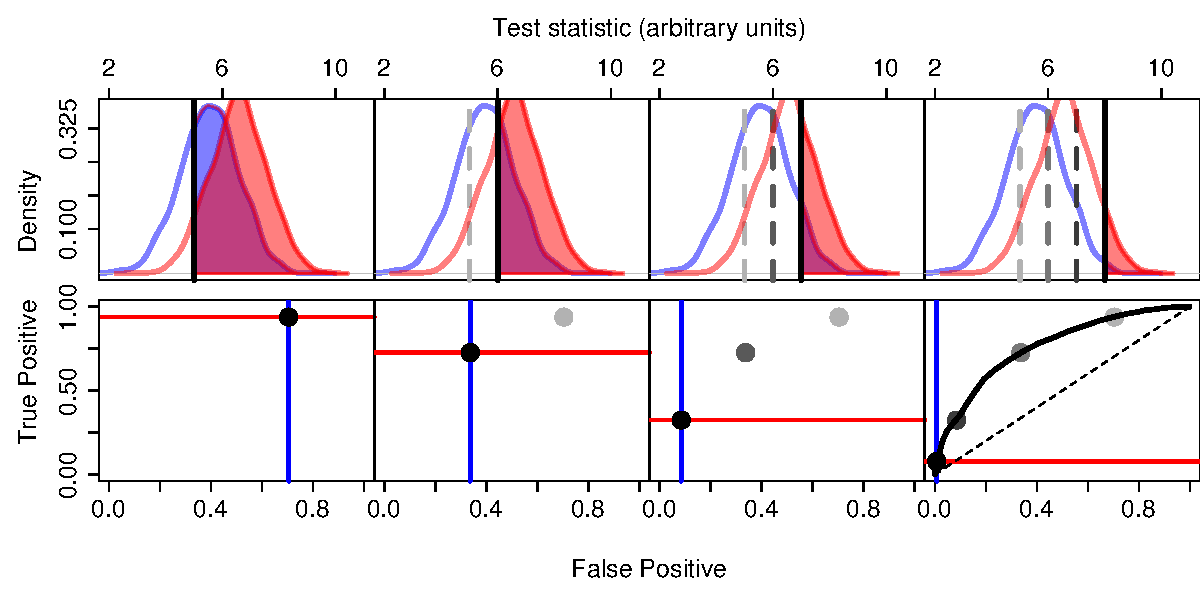
\includegraphics[width=\linewidth]{Fig1}
     \label{fig:fig1}
     \caption{Top row: The distributions of a hypothetical warning indicator are shown under the case of a stable system (blue) and a system approaching a critical transition (red).  Bottom row: Points along the ROC curve are calculated for each possible threshold indicated in the top row.  The false positive rate is the integral of the distribution of the test statistic under the stable system right of the threshold (blue shaded area, corresponding to blue vertical line).  The true positive rate is the integral of the system approaching a transition left of the threshold (red shaded area, corresponds to the red line).  Successive columns show the threshold increasing, tracing out the ROC curve.}
  \end{center}
 \end{figure}



 \begin{figure}[h]
   \begin{center}
     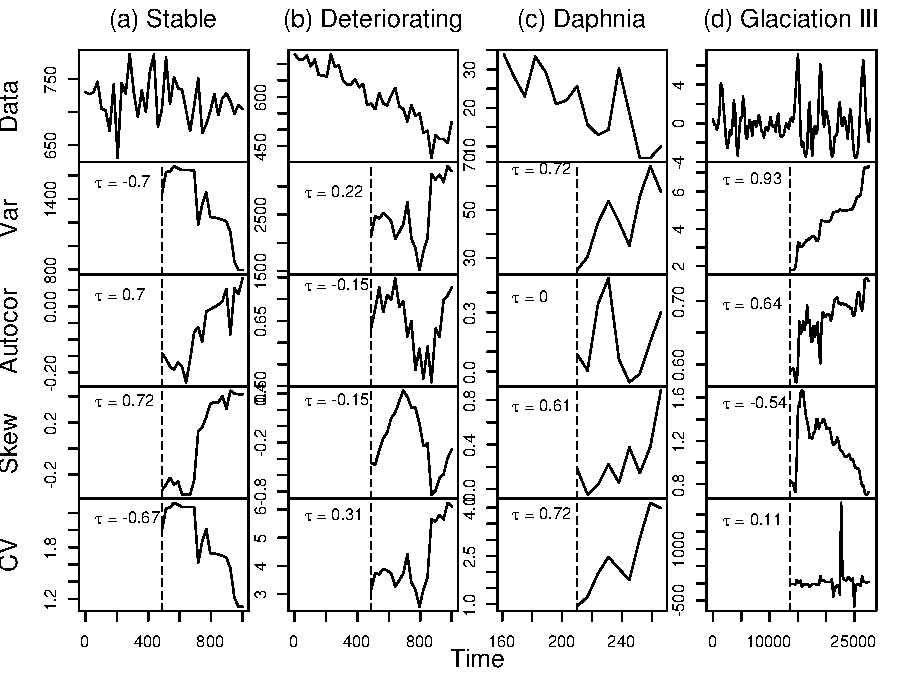
\includegraphics[width=\linewidth]{Fig2}
     \label{fig:fig2}
     \caption{Early warning signals in simulated and empirical data sets.  The first two columns are simulated data from (a) a stable system (Stable), and (b) the same system approaching a saddle-node bifurcation (Deteriorating).  Empirical examples are from (c) \emph{Daphnia magna} concentrations manipulated towards a critical transition (Daphnia), and (d) deuterium concentrations previously cited as an early warning signal of a glaciation period (Glaciation). Increases in summary statistics, computed over a moving window, have often been used to indicate if a system is moving towards a critical transition.  The increase is measured by the correlation coefficient $\tau$.  Note that positive correlation does not guarantee the system is moving towards a transition, as seen in the stable system, first column.}
  \end{center}
 \end{figure}



 \begin{figure}[h]
   \begin{center}
     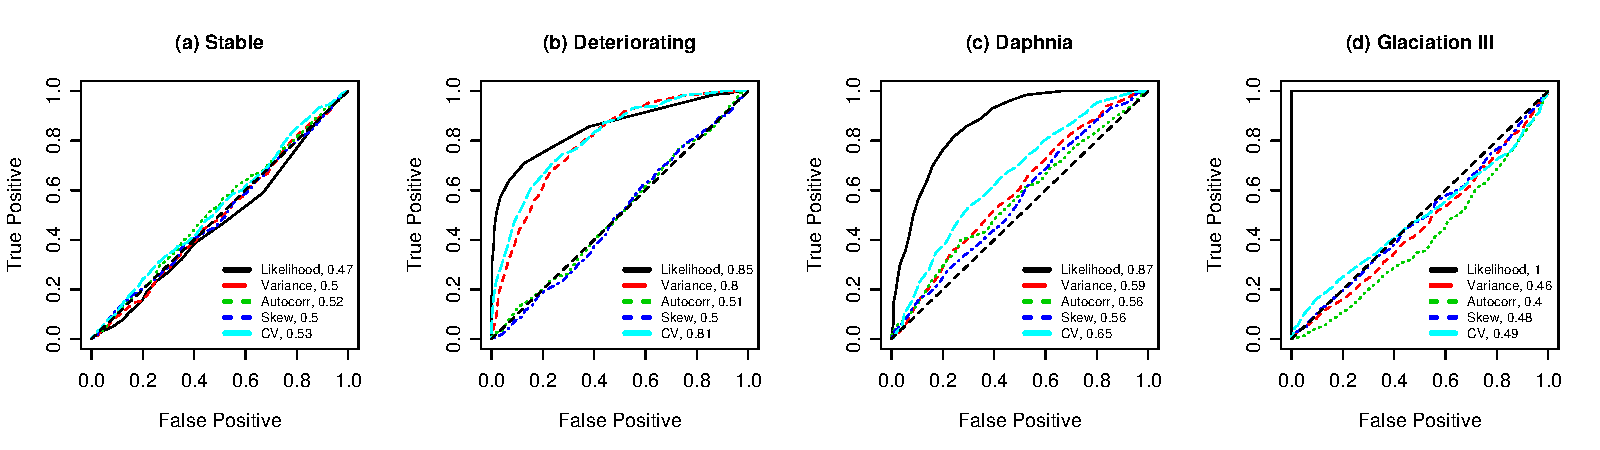
\includegraphics[width=\linewidth]{Fig3.pdf}
     \label{fig3}
     \caption{ROC curves for different early warning indicators on simulated and empirical data.  The area under the curve, inset, indicates how the method compares to a random guess (0.5).  The likelihood method performs substantially better than other metrics, particularly on the weaker trends seen in the empirical data. The simulated data sets have 40 points, ``Daphnia'' has 16, the ``Glaciation'' has 121. See corresponding distributions, Fig. S1.}
  \end{center}
 \end{figure}


 \begin{figure}[h!]
   \begin{center}
     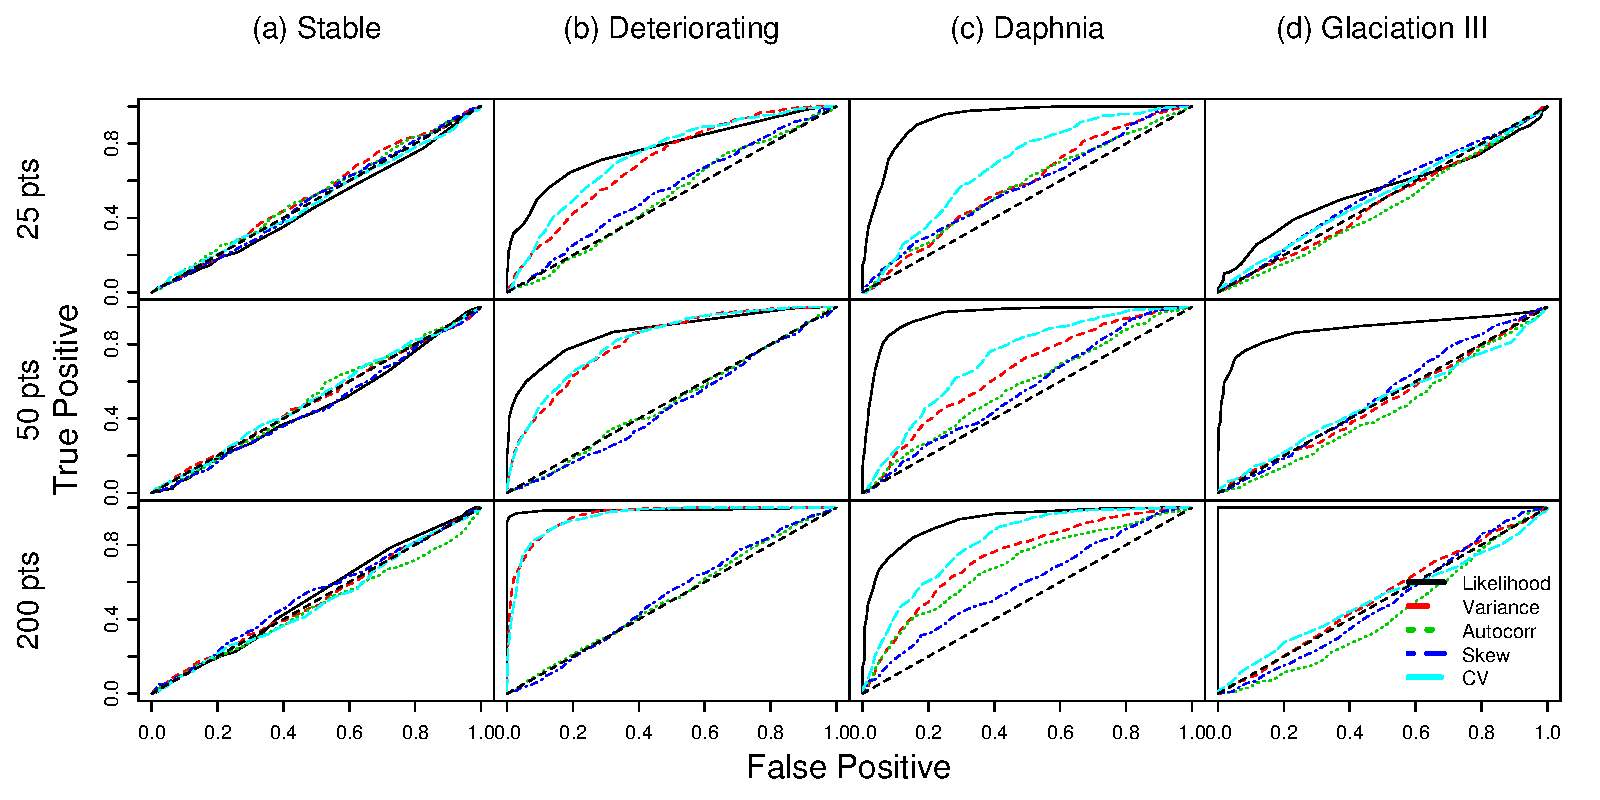
\includegraphics[width=\linewidth]{Fig4.pdf}
     \label{fig4}
     \caption{ROC curves (from Fig. 3) are recalculated under different sampling frequencies in the simulation step (see supplementary online text), using a total of 25, 50, or 200 points.  Increasing the sampling improves the trade-off between sensitivity and reliability for all indicators, though the likelihood approach is most effective. A warning signal is not detected in stable system simulation. Corresponding distributions shown in Fig S2-5.} 
  \end{center}
 \end{figure}

 \end{document}



